\section{Frontend}

Per interagire con il sistema, gli utenti utilizzano una WebApp sviluppata interamente dal mio collega di tirocinio. Il mio contributo è stato principalmente fornire l'infrastruttura necessaria per il deployment dell'applicazione. 
Come anticipato nella sezione

Di seguito è riportato un diagramma che illustra i principali servizi e utenti che interagiscono con questa parte del sistema:

\begin{figure}[ht]  
    \centering
    \makebox[\textwidth][c]{%
        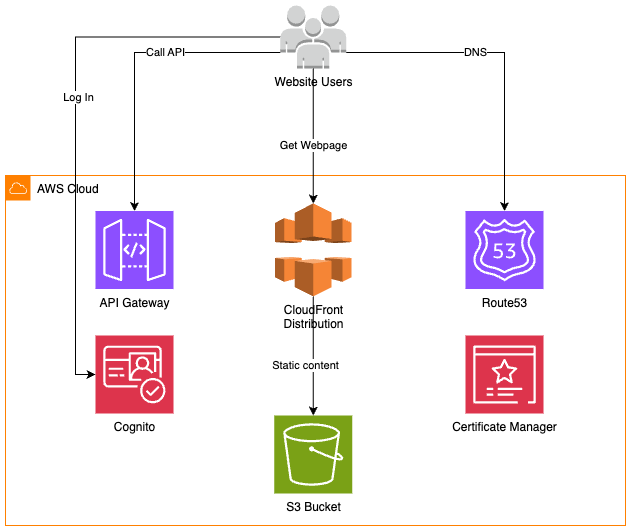
\includegraphics[width=0.8\linewidth]{immagini/infra/frontend.png}%
    }
    \caption{Architettura frontend nel tettaglio}
    \label{imm:infra_frontend}
\end{figure}

\FloatBarrier

-- qui manca da qualche parte il riferimento al "contratto" fatto con la specifica openapi, e che nel mentre dello sviluppo abbiamo aggiunto funzionalita rilevate necessarie

La WebApp è stata sviluppata utilizzando React, il che significa che è stata implementata come una single-page application (SPA). Una SPA è caratterizzata dal fatto che, per ottenere l'intera applicazione, è sufficiente ricevere i file statici iniziali, i quali includono il routing interno e le chiamate alle API per popolare le interfacce utente. Questo approccio elimina la necessità di un server per elaborare dinamicamente le pagine in base alle richieste degli utenti, poiché tale elaborazione avviene sul lato client.

Inizialmente, si era considerato l'utilizzo di \texttt{Next.js}, un framework fullstack per creare applicazioni web che sfrutta React come libreria client. Questo framework avrebbe offerto la possibilità di caricare le pagine ibridamente, sia lato server che lato client, garantendo una maggiore flessibilità. Tuttavia, questa soluzione non era in linea con i requisiti serverless del progetto di tirocinio. Inoltre, l'adozione di Next.js avrebbe comportato un aumento della complessità del sistema, introducendo la necessità di gestire un server aggiuntivo. Considerando che le funzionalità del servizio non richiedevano un approccio così avanzato, l'utilizzo di Next.js non sembrava giustificato.

\vspace{0,3cm}

La \texttt{distribuzione} della WebApp è stata fatta tramite \texttt{CloudFront}, un Content Delivery Network (CDN) progettato per distribuire in modo efficiente contenuti statici su scala globale.
La nostra Web App utilizza un Bucket \texttt{S3} (Simple Storage Service) per immagazzinare la build del frontend. CloudFront agisce come uno strato di distribuzione globale che si interpone tra l'utente finale e il Bucket S3. 

-- qui manca la valutazione di amplify


Per quanto riguarda l'autenticazione con il sistema dalla WebApp, rimando alla sezione \ref{autenticazione}.